\documentclass{beamer}

\usepackage{lmodern}

\usepackage{algorithm}
\usepackage{algpseudocode}


\title{Creation of Polygons}
\subtitle{Randomly}
\author{Christoph Ladurner}
\date{21.06.2018}

\begin{document}

\begin{frame}
  \titlepage
\end{frame}

\begin{frame}
  The first three algorithms are
  \begin{enumerate}
    \item Randomly created point cloud
    \item Regular polygon
    \item Fix Local Orientation
  \end{enumerate}

  They have in common
  \begin{enumerate}
    \item They are used as starting point for other algorithms.
    \item They are created with only the settings as input
  \end{enumerate}
\end{frame}

\begin{frame}{Randomly created point cloud}
  \begin{block}{}
    \begin{columns}[onlytextwidth,T]
      \column{\dimexpr\linewidth-40mm}
      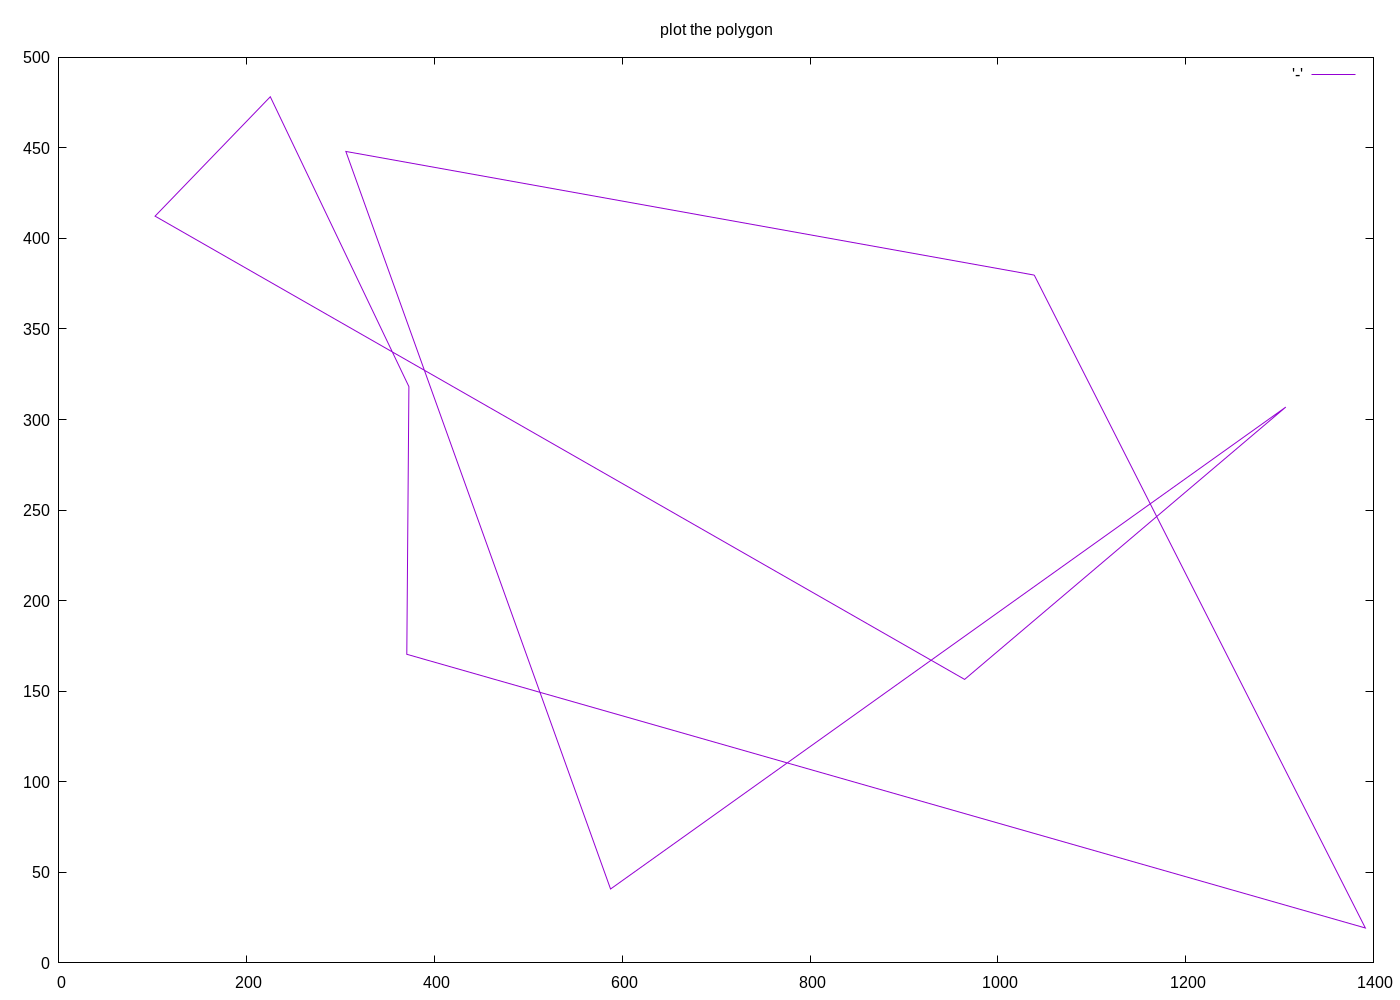
\includegraphics[width=0.5\paperwidth]{figures/kk-random-10-0-0.png}
      \column{40mm}
      This shows a polygon with randomly created points.
    \end{columns}
  \end{block}
\end{frame}

\begin{frame}{Randomly created point cloud Pseudocode}
  \begin{algorithm}[H]
    \begin{algorithmic}[0]
      \Procedure{$random$}{$N, area$}
        \State $r\gets createRandomValueGenerator(area)$
        \State $list \gets []$
        \For {$i \leftarrow 1 \cdots N$}
          \State $x \gets r()$
          \State $y \gets r()$
          \State $list \gets list + \{x,y\}$
        \EndFor
        \State \textbf{return} $list$
      \EndProcedure
    \end{algorithmic}
  \end{algorithm}
\end{frame}

\begin{frame}{Regular Polygon}
  \begin{block}{}
    \begin{columns}[onlytextwidth,T]
      \column{\dimexpr\linewidth-40mm}
      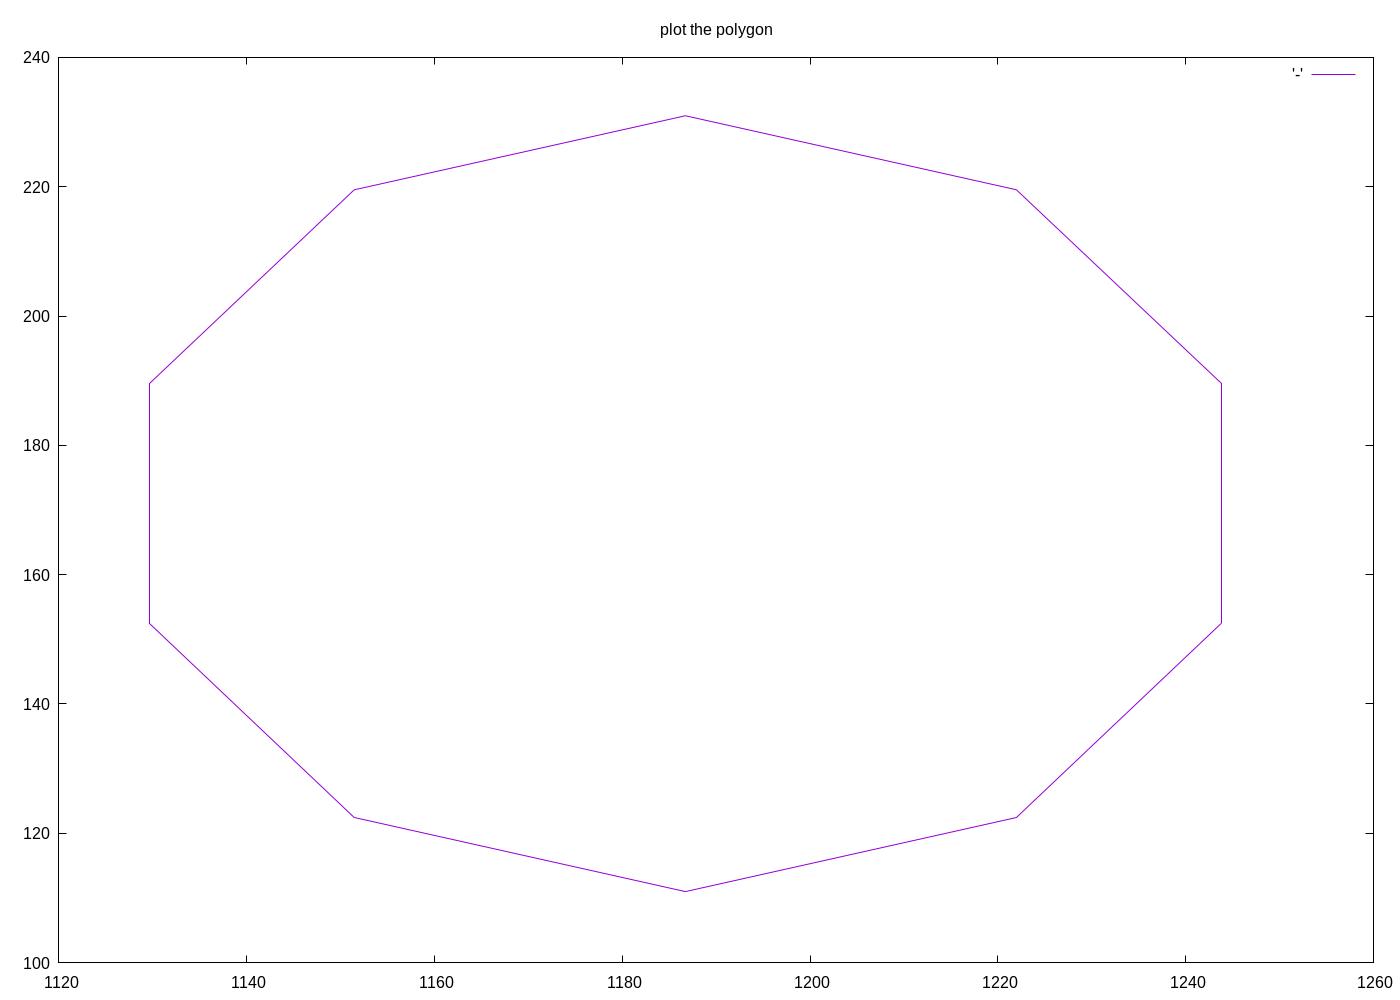
\includegraphics[width=0.5\paperwidth]{figures/kk-regular-polygon-10-0-0.png}
      \column{40mm}
      The regular polygon is a simple polygon which forms the polygon with
      points rotated around a center with a fixed radius and a fixed angle.
    \end{columns}
  \end{block}
\end{frame}

\begin{frame}{Regular Polygon Pseudocode}
  \begin{algorithm}[H]
    \begin{algorithmic}[0]
      \Procedure{$regularPolygon$}{$settings$}
        \State $angle \gets 2 * \pi * 1 / N$
        \State $polygon \gets []$
        \For {$i \leftarrow 1 \cdots N$}
          \State $x \gets radius * cos(i * angle) + center.x$;
          \State $y \gets radius * sin(i * angle) + center.y$;
          \State $polygon \gets polygon + \{x,y\}$
        \EndFor
        \State \textbf{return} $polygon$
      \EndProcedure
    \end{algorithmic}
  \end{algorithm}
\end{frame}

\begin{frame}{Fix Local Orientation}
  \begin{block}{}
    \begin{columns}[onlytextwidth,T]
      \column{\dimexpr\linewidth-40mm}
      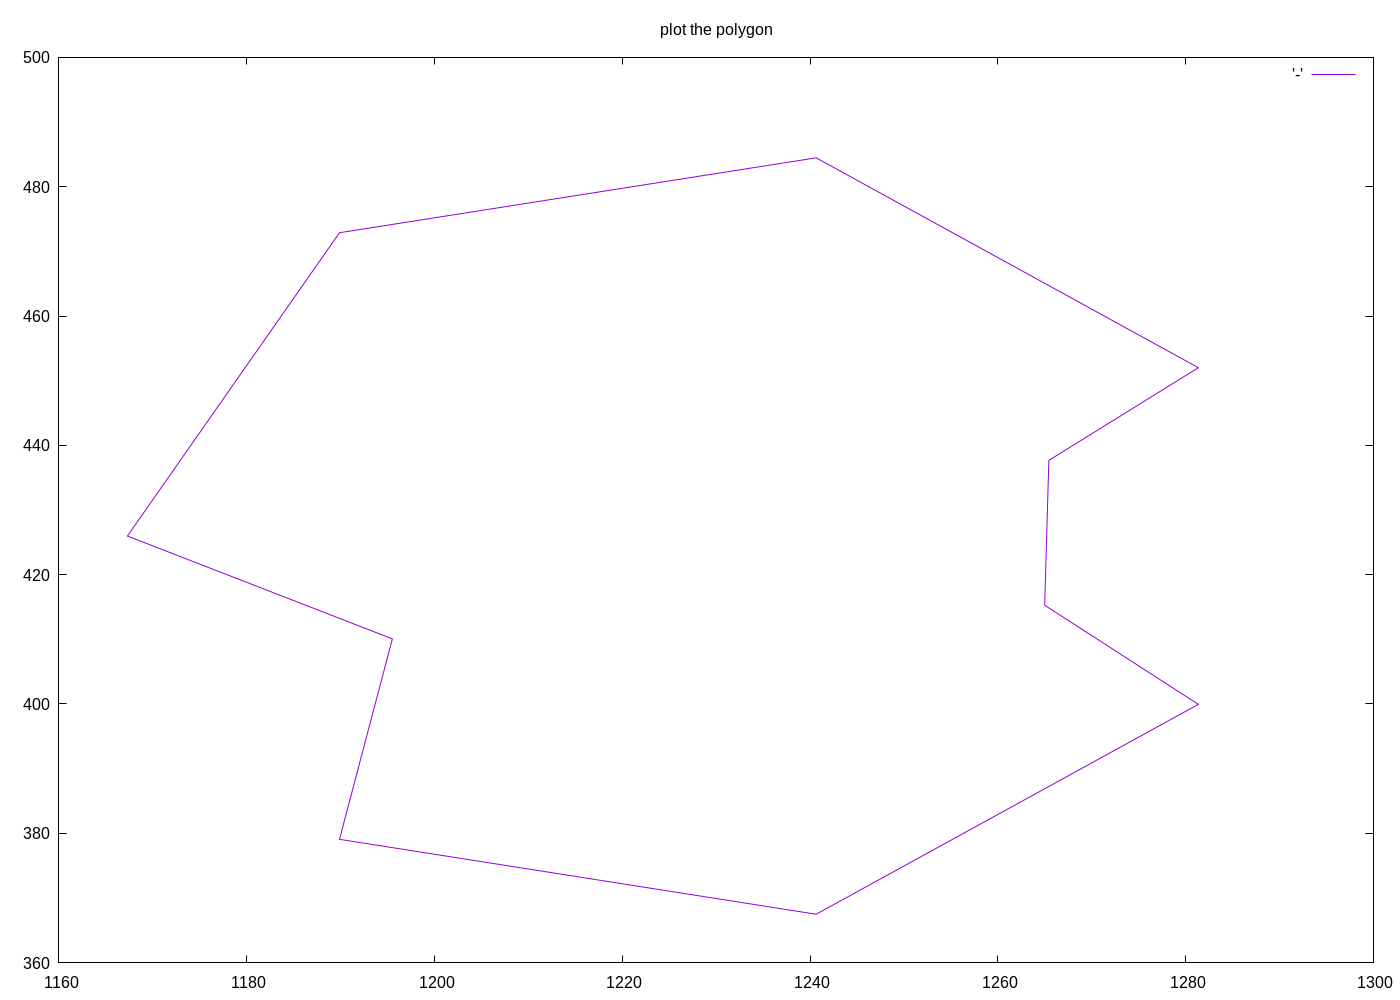
\includegraphics[width=0.5\paperwidth]{figures/kk-fix-local-orientation-10-3-0.png}
      \column{40mm}
      This algorithm is a further stage of the regular polygon which offers the
      possibility to add reflex nodes to the simple polygon. It uses the
      Thales's theorem.
    \end{columns}
  \end{block}
\end{frame}

\begin{frame}{Fix Local Orientation Pseudocode}
  \begin{algorithm}[H]
    \scriptsize
    \begin{algorithmic}[0]
      \Procedure{$fixLocalOrientation$}{$settings$}
        \State $polygon \gets regularPolygon$
        \State $reflexPointsPerSegment \gets initReflexPoints(settings)$
        \For {$i \leftarrow 1 \cdots Segments$}
          \State $reflexPoints \gets createReflexPointsOnInnerArc(reflexPointsPerSegment[i])$
          \State $polygon \gets polygon[i] + reflexPoints$
        \EndFor
        \State \textbf{return} $polygon$
      \EndProcedure
      \vspace{3pt}
      \Procedure{$createReflexPointsOnInnerArc$}{$settings$}
        \State $reflexCircleCenter \gets search\ center\ of\ segment$
        \State $rotationVec \gets segments.target() - reflexCircleCenter$
        \State $angle \gets 2*\pi*1/reflexPointsPerSegment$
        \For {$i \leftarrow 1 \cdots reflexNodes$}
          \State $reflexPos \gets reflexCircleCenter + rotate(rotationVex, angle)$
          \State $reflexPoints \gets reflexPoints + reflexPos$
        \EndFor
        \State \textbf{return} $reflexPoints$
      \EndProcedure
    \end{algorithmic}
  \end{algorithm}
\end{frame}


\begin{frame}{}
  The following algorithms starts the calculation of the simple
  polygon with a randomly created point cloud.

  \begin{enumerate}
    \item Random Two Peasants
    \item Convex Bottom
    \item Steady Growth
    \item Space Partitioning
    \item 2-Opt Moves
  \end{enumerate}
\end{frame}

\begin{frame}{Random Two Peasants}
  \begin{block}{}
    \begin{columns}[onlytextwidth,T]
      \column{\dimexpr\linewidth-40mm}
      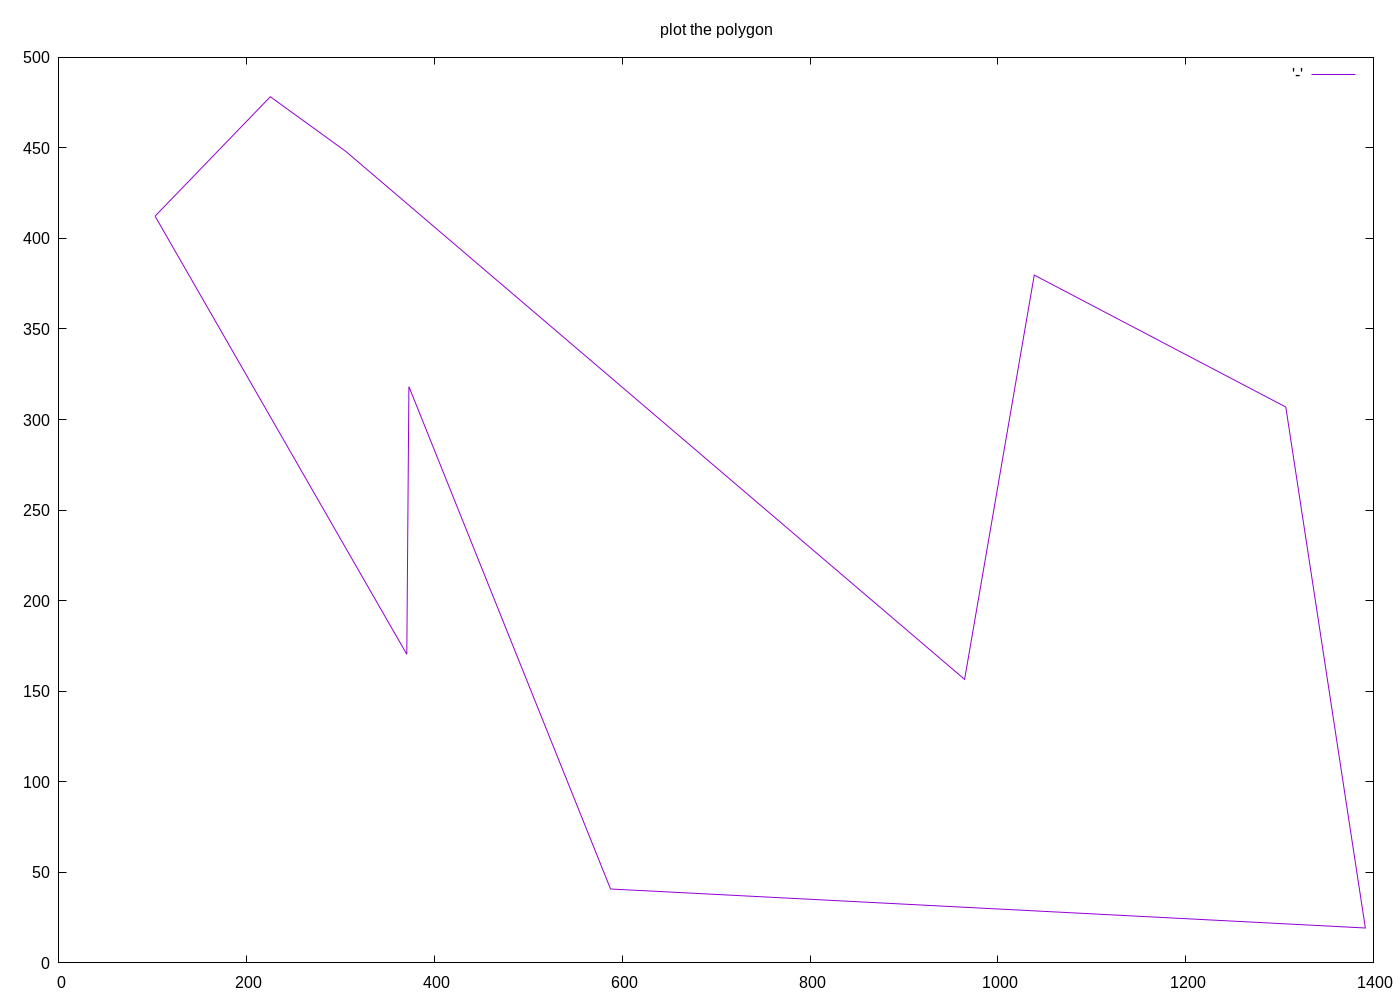
\includegraphics[width=0.5\paperwidth]{figures/kk-random-two-peasants-10-0-0.png}
      \column{40mm}
      Random Two Peasants divides the point cloud in two separate groups by a line throw
      the lowest and the highest point on x-axis. The upper group is used to
      initialize the polygon, the group below the line is added in reverse order
      to the polygon.
    \end{columns}
  \end{block}
\end{frame}

\begin{frame}{Random Two Peasants Pseudocode}
  \begin{algorithm}[H]
    \begin{algorithmic}[0]
      \Procedure{$randomTwoPeasants$}{$list$}
        \State $list \gets sort(list)$
        \State $min \gets first(list)$
        \State $max \gets last(list)$
        \State $divide\ list\ by\ line(min,\ max)$
        \State $polygon \gets upper$
        \State $polygon \gets reverse(bottom)$
        \State \textbf{return} $polygon$
      \EndProcedure
    \end{algorithmic}
  \end{algorithm}
\end{frame}

\begin{frame}{Convex Bottom}
  \begin{block}{}
    \begin{columns}[onlytextwidth,T]
      \column{\dimexpr\linewidth-40mm}
      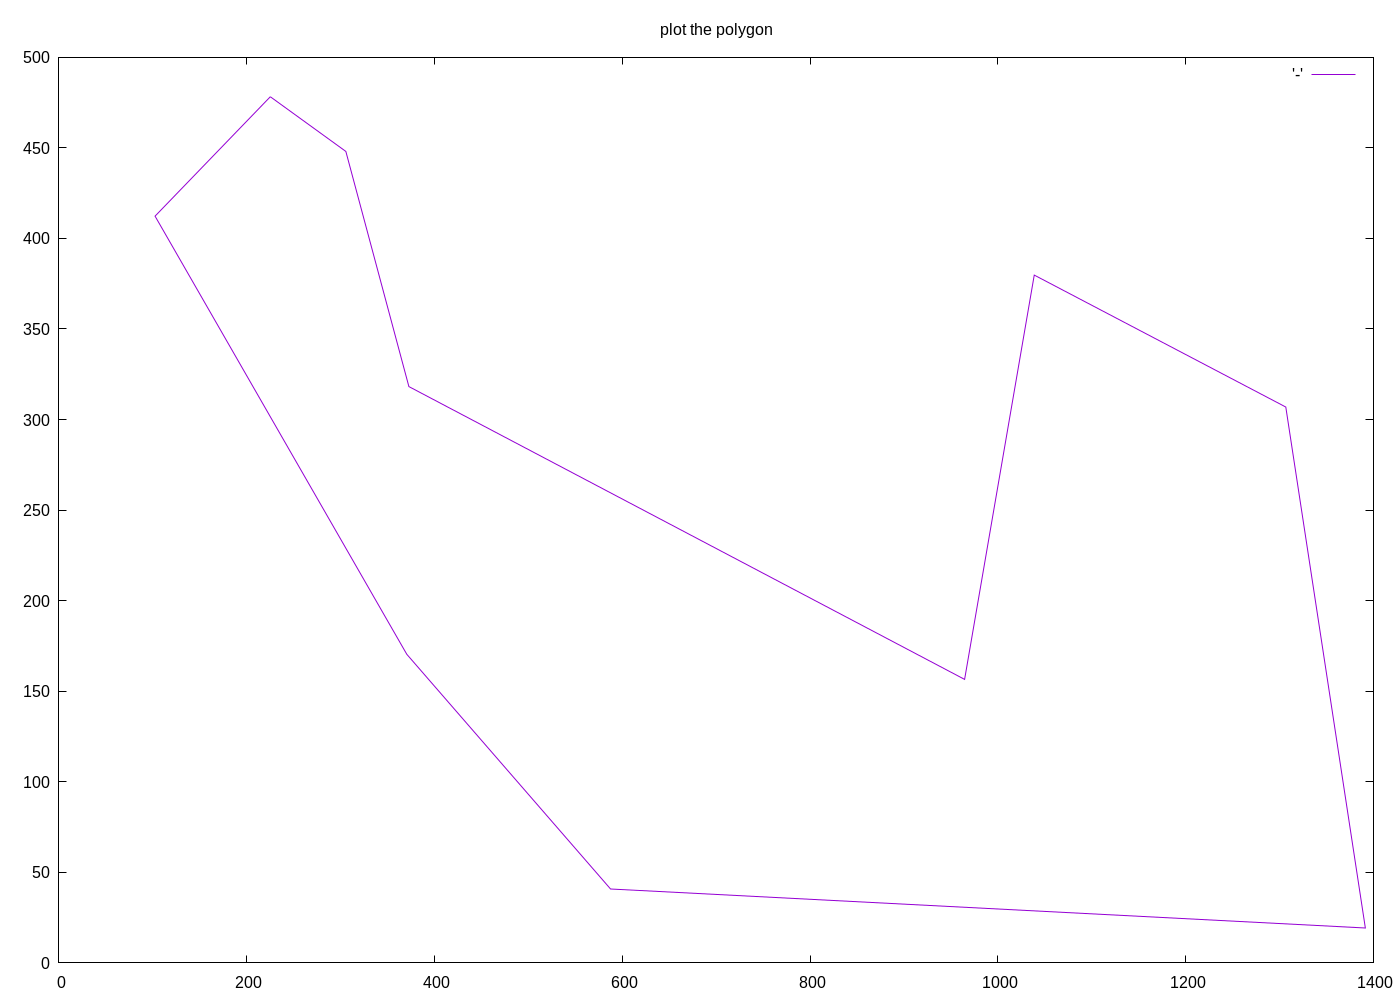
\includegraphics[width=0.5\paperwidth]{figures/kk-convex-bottom-10-0-0.png}
      \column{40mm}
      \small
      The convex bottom algorithm divides the point cloud in two separated
      groups by a line throw the lowest and highest point on the x-axis. the
      bottom group is used to create a convex hull. all points not on that
      convex hull are sorted on x-axis and then added to the polygon and the
      convex hull in reverse order.
    \end{columns}
  \end{block}
\end{frame}

\begin{frame}{Convex Bottom Pseudocode}
  \begin{algorithm}[H]
    \begin{algorithmic}[0]
      \Procedure{$convexBottom$}{$list$}
        \State $list \gets sort(list)$
        \State $min \gets first(list)$
        \State $max \gets last(list)$
        \State $divide\ list\ by\ line(min,\ max)$
        \State $convex\_hull \gets createConvexHull(bottom)$
        \For {$i \leftarrow 1 \cdots N$}
          \If {$point\ not\ on\ hull$}
            \State $polygon \gets polygon + point$
          \EndIf
        \EndFor
        \State $polygon \gets reversed(convex\_hull)$
        \State \textbf{return} $polygon$
      \EndProcedure
    \end{algorithmic}
  \end{algorithm}
\end{frame}

\begin{frame}{Steady Growth}
  \begin{block}{}
    \begin{columns}[onlytextwidth,T]
      \column{\dimexpr\linewidth-40mm}
      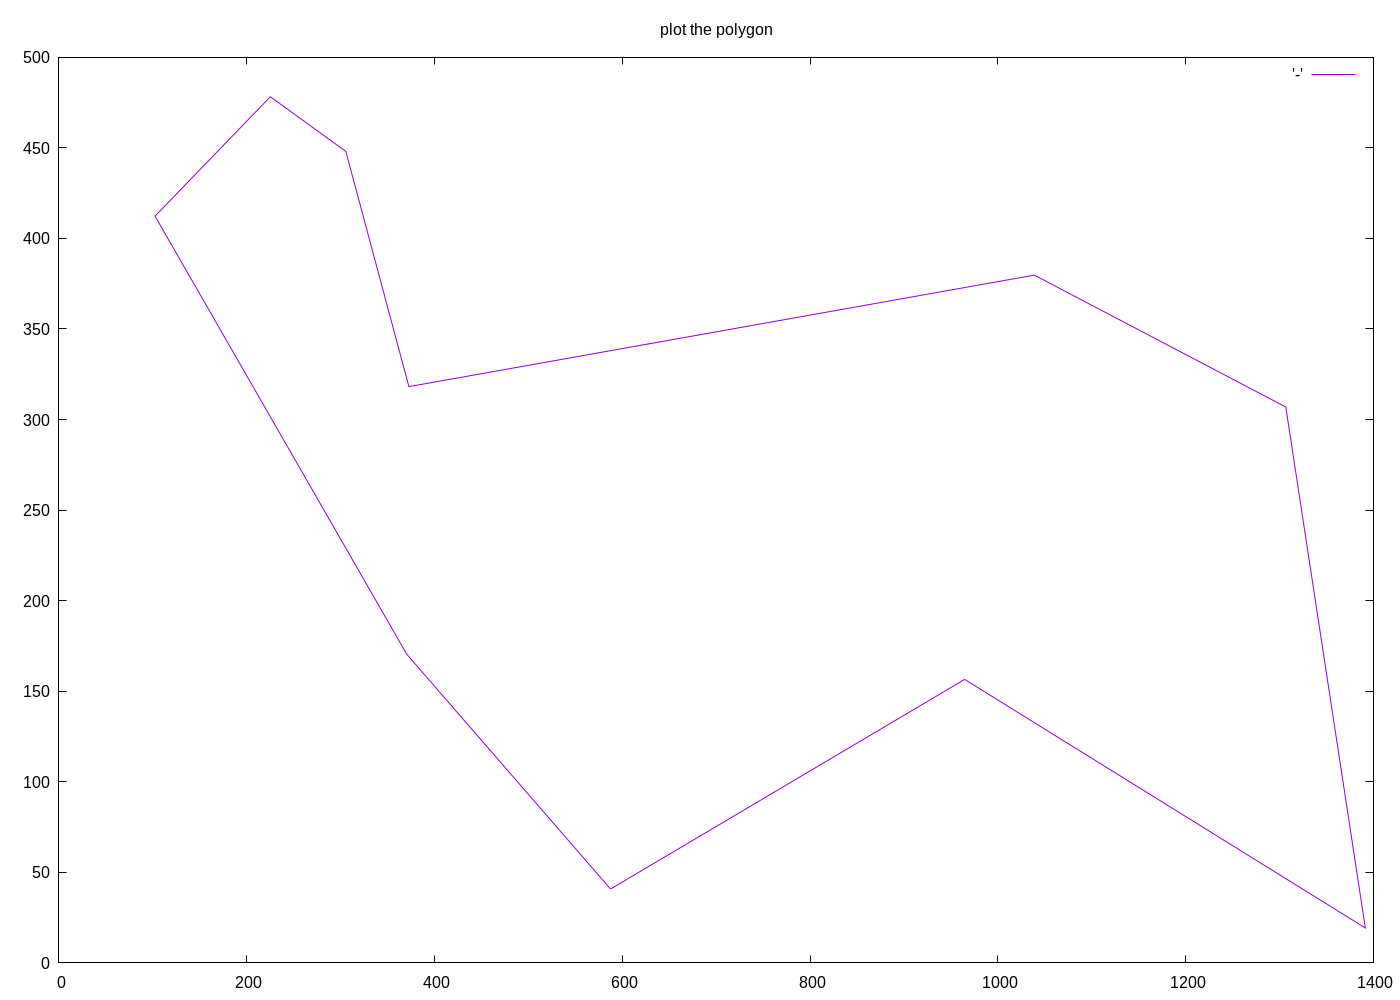
\includegraphics[width=0.5\paperwidth]{figures/kk-steady-growth-10-0-0.png}
      \column{40mm}
      This algorithm use a convex hull to find the support vertices (SV) of the choosen
      random point. The SV are used to check if no other point lies within the
      triangle of SV and the point. The SV are also used to find a complete
      visible segment to add the new point to the polygon.
    \end{columns}
  \end{block}
\end{frame}

\begin{frame}{Steady Growth Pseudocode}
  \begin{algorithm}[H]
    \scriptsize
    \begin{algorithmic}[0]
      \Procedure{$steadyGrowth$}{$list$}
        \State $s_1, s_2 \gets locateTwoIndependendPoints(list)$
        \State $convexHull = \{s_1, s_2\}; final = \{s_1, s_2\}$
        \For {$i \leftarrow 1 \cdots N$}
          \State $p \gets locateRandomPoint(list, convexHull)$
          \State $segment \gets locateVisibleSegment(final, p)$
          \State $replaceSegment(final, segment, p)$
          \State $addToConvexHull(convexHull, p)$
        \EndFor
        \State \textbf{return} $polygon$
      \EndProcedure
      \vspace{3pt}
      \Procedure{$locateRandomPoint$}{$list, convexHull$}
        \State $p \gets select(list)$
        \State $s_l, s_r \gets locateSupportVertices(convexHull, p)$
        \For {$i \leftarrow 1 \cdots N$}
          \If {$point\ inside\ triangle s_l, s_r, p$}
            \State $recalculate\ support\ vertices$
          \EndIf
        \EndFor
        \State \textbf{return} $p$
      \EndProcedure
    \end{algorithmic}
  \end{algorithm}
\end{frame}

\begin{frame}{Space Partitioning}
  \begin{block}{}
    \begin{columns}[onlytextwidth,T]
      \column{\dimexpr\linewidth-40mm}
      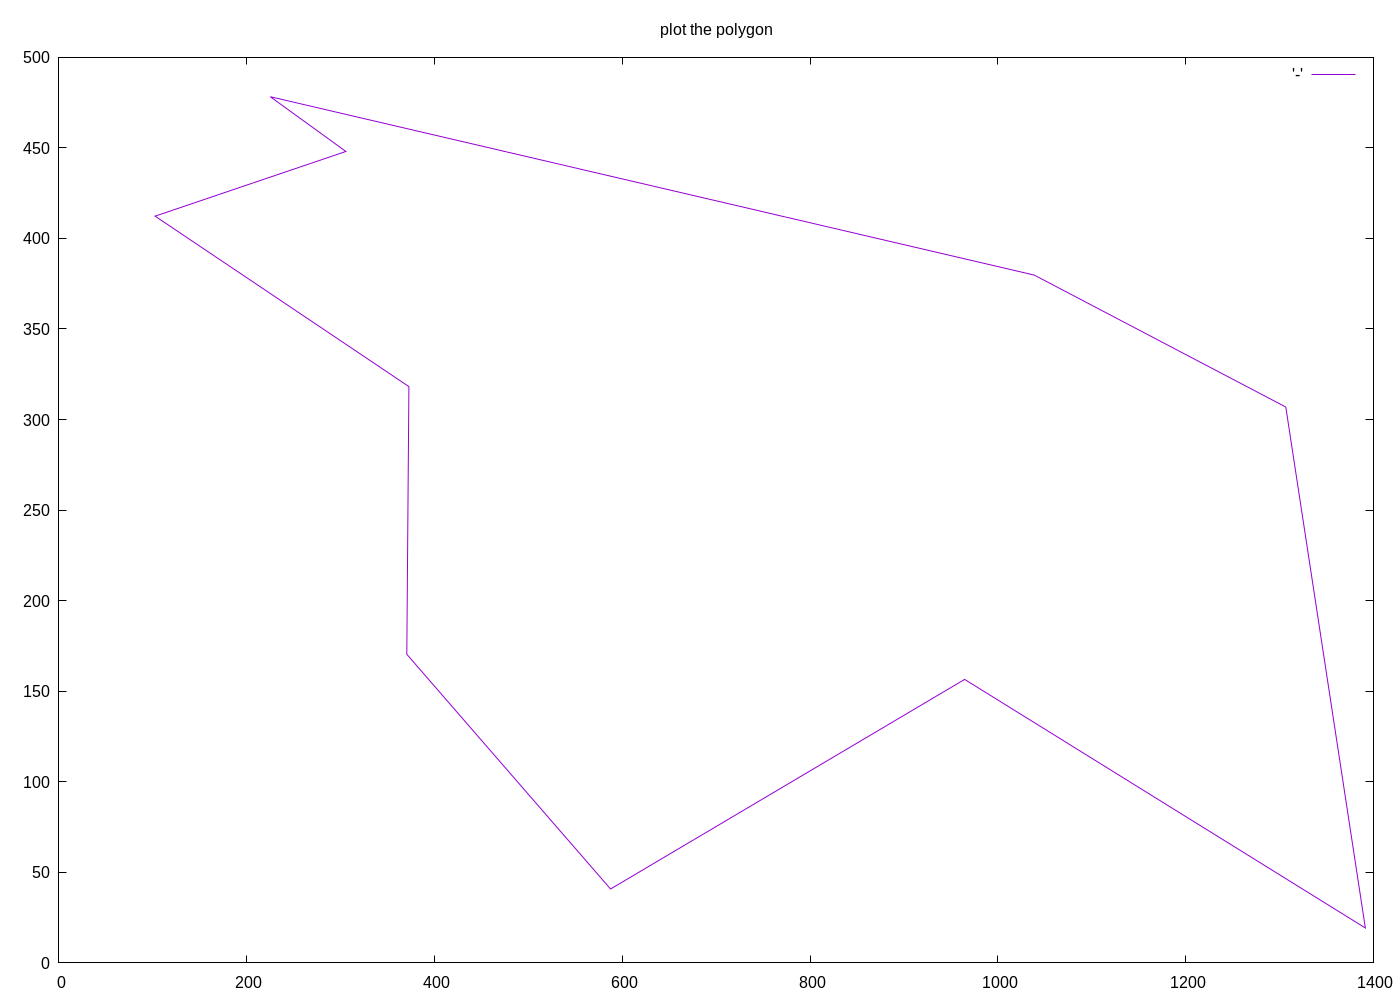
\includegraphics[width=0.5\paperwidth]{figures/kk-space-partitioning-10-0-0.png}
      \column{40mm}
      The key points on this algorithm is the recursive approach and the
      ensuring that every line used to separate the groups has the same
      direction to construct the polygon recursively.
    \end{columns}
  \end{block}
\end{frame}

\begin{frame}{Space Partitioning Pseudocode}
  \begin{algorithm}[H]
    \scriptsize
    \begin{algorithmic}[0]
      \Procedure{$spacePartitioning$}{$list$}
        \State $s_f,s_l \gets chooseRandomPoints(list)$ \Comment{$s_f < s_l$}
        \State $S_f, S_l \gets divide\ list\ by\ line(s_f, s_l)$
        \State \Call{$recursiveDivide$}{$S_f, s_f, s_l, polygon$}
        \State \Call{$recursiveDivide$}{$S_l, s_l, s_f, polygon$}
        \State \textbf{return} $polygon$
      \EndProcedure
      \vspace{3pt}
      \Procedure{$recursiveDivide$}{$S, s_f, s_l, polygon$}
        \If {$S.size == 2$}
          \State $polygon \gets polygon + s_l$
        \ElsIf {$S.size == 3$}
          \State $polygon \gets polygon + s$ \Comment{$s \neq s_l \land s \neq s_f$}
          \State $polygon \gets polygon + s_l$
        \Else
          \State $s \gets calculateRandomPoint(S, s_f, s_l)$
          \State $l \gets calculateRandomLine(s, s_f, s_l)$
          \State $S_f, S_l \gets divide\ list\ by\ line(s_f, s_l)$
          \State \Call{$recursiveDivide$}{$S_f, s_f, s_l, polygon$}
          \State \Call{$recursiveDivide$}{$S_l, s_l, s_f, polygon$}
        \EndIf
      \EndProcedure
    \end{algorithmic}
  \end{algorithm}
\end{frame}

\begin{frame}{2-Opt Moves}
  \begin{block}{}
    \begin{columns}[onlytextwidth,T]
      \column{\dimexpr\linewidth-40mm}
      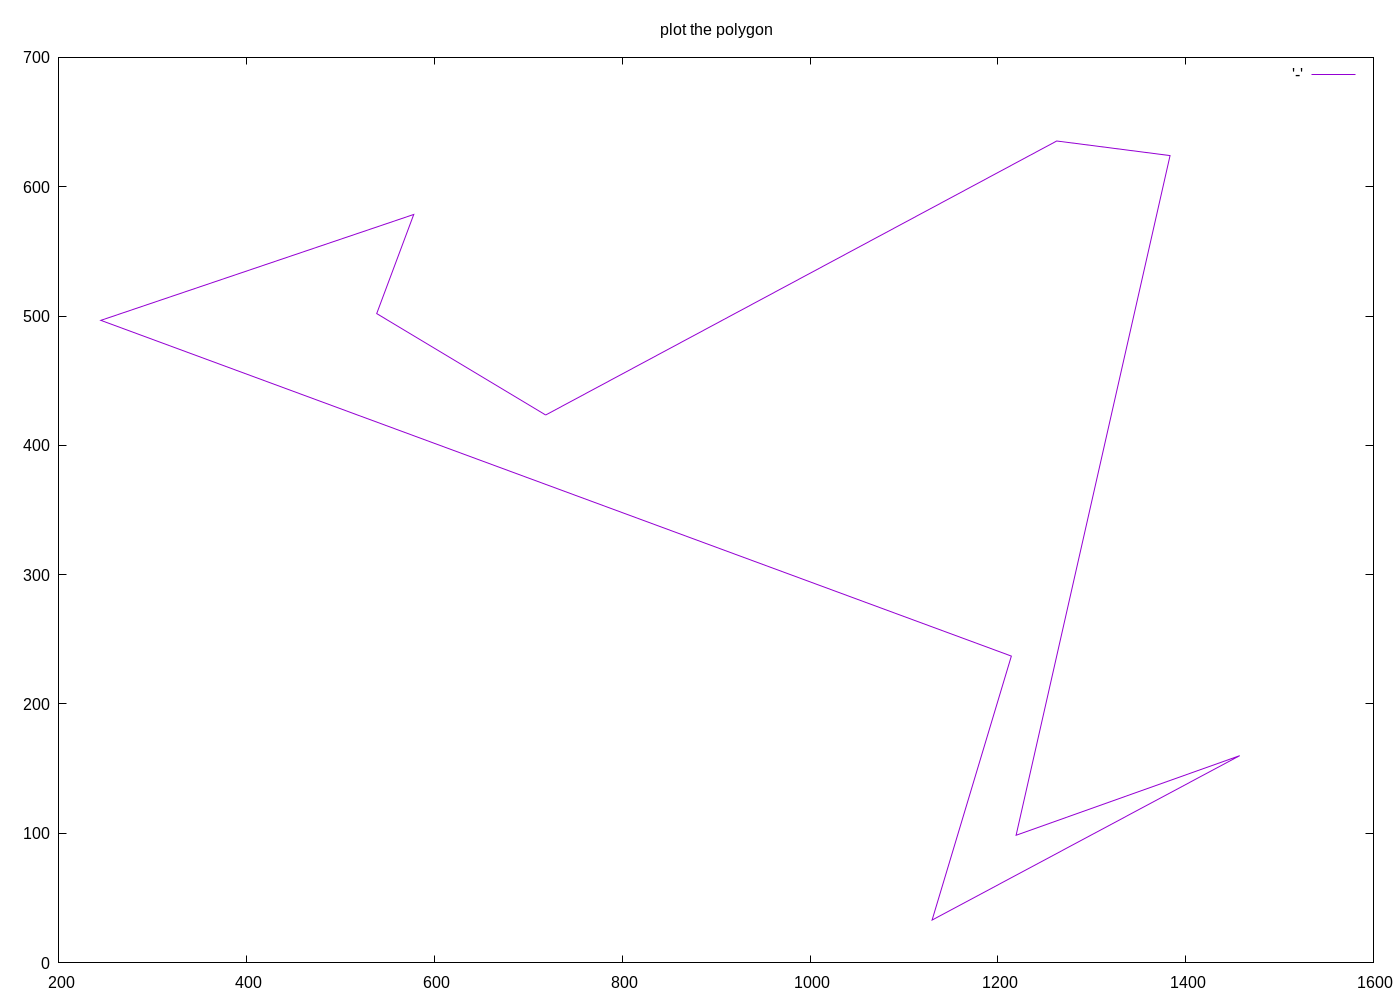
\includegraphics[width=0.5\paperwidth]{figures/kk-two-opt-moves-10-0-0.png}
      \column{40mm}
      The 2-Opt Moves algorithm calculates all intersections from a random
      polygon and resvoles it in a next step. Then it calculates the new created
      intersections and resolves that and so on.
    \end{columns}
  \end{block}
\end{frame}

\begin{frame}{2-Opt Moves Pseudocode}
  \begin{algorithm}[H]
    \tiny
    \begin{algorithmic}[0]
      \Procedure{$twoOptMoves$}{$list$}
        \State $intersections \gets calculateIntersections(list)$
        \State $resolveIntersections(segments, intersections)$
        \State $polygon \gets calculateFinalList(segments)$
        \State \textbf{return} $polygon$
      \EndProcedure

      \Procedure{$calculateIntersections$}{$segments$}
        \For {$s_1 \leftarrow 1,segments$}
          \For {$s_2 \leftarrow 1,segments$}
            \If {$isIntersection(s_1, s_2) and isUnique(intersections, s_1, s_2)$}
              \State $intersections \gets intersections + \{s_1, s_2\}$
            \EndIf
          \EndFor
        \EndFor
      \EndProcedure

      \Procedure{$resolveIntersections$}{$segments, intersections$}
        \For {$s_1 \leftarrow 1,intersections$}
          \State $intersection \gets select(intersections)$
          \State $removeIntersection$
          \State $e_1, e_2 \gets calculateNewSegment$
          \State $calculate\ all\ new\ intersections$
          \State $segments \gets segments + e_1 + e_2$
        \EndFor
      \EndProcedure
    \end{algorithmic}
  \end{algorithm}
\end{frame}

\begin{frame}{}
  \centering \Large
  Algorithms without random point cloud as start point
\end{frame}

\begin{frame}{Bouncing Vertices}
  \begin{block}{}
    \begin{columns}[onlytextwidth,T]
      \column{\dimexpr\linewidth-40mm}
      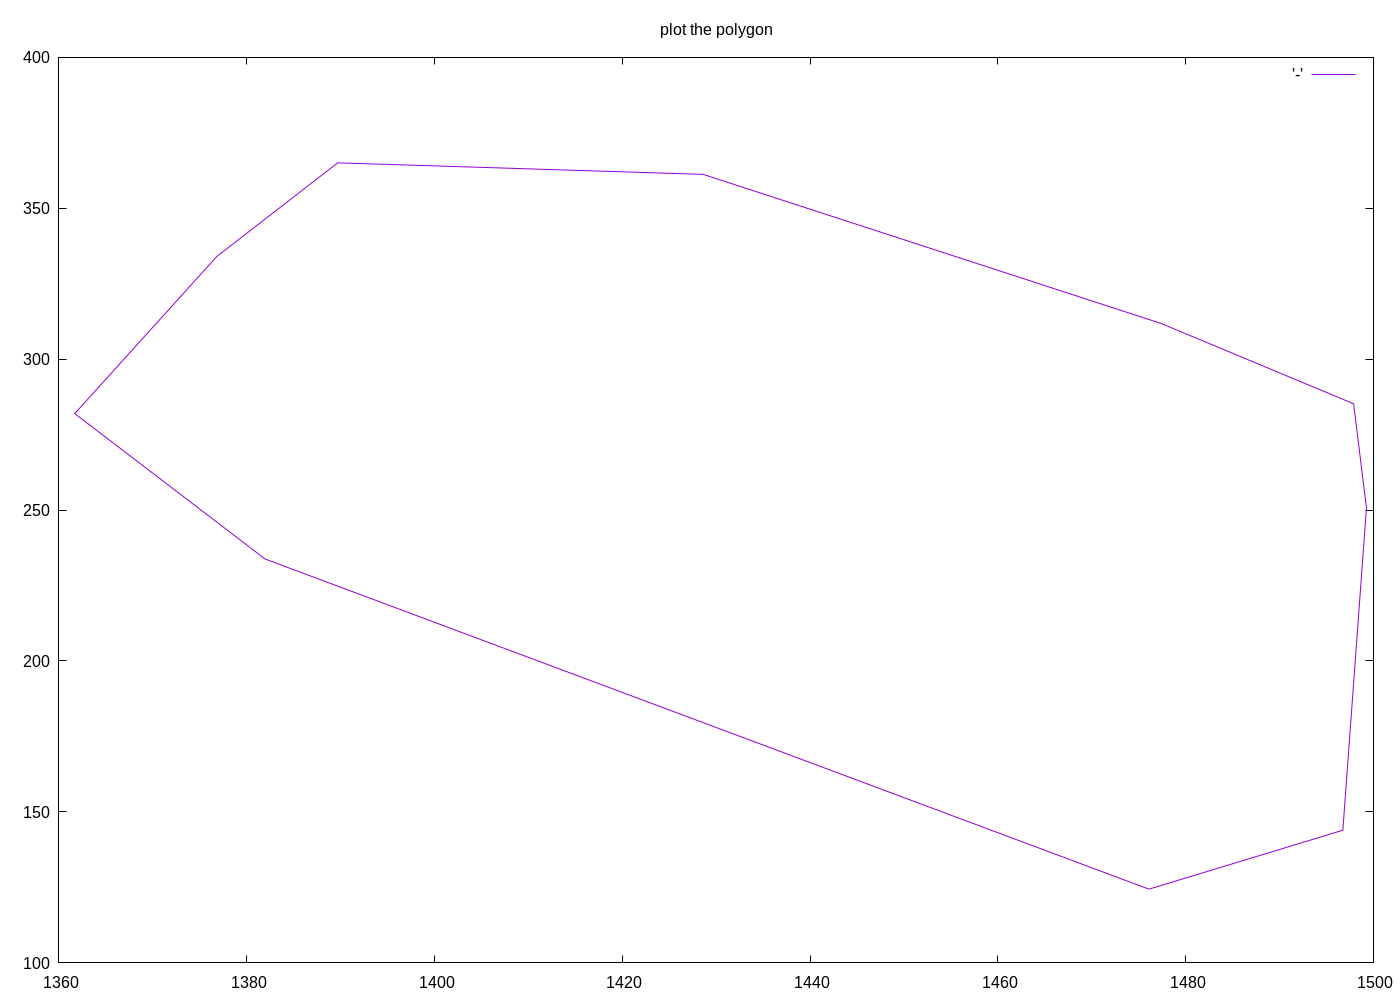
\includegraphics[width=0.5\paperwidth]{figures/kk-bouncing-vertices-10-0-0.png}
      \column{40mm}
      Use a simple polygon and bounce every point k times around in a way, that
      the simple states remains.
    \end{columns}
  \end{block}
\end{frame}

\begin{frame}{Bouncing Vertices Pseudocode}
  \begin{algorithm}[H]
    \tiny
    \begin{algorithmic}[0]
      \Procedure{$bouncingVertices$}{$simplePolygon, settings$}
        \For {$i \leftarrow 1 \cdots k$}
          \For {$i \leftarrow 1 \cdots N$}
            \State $newPoint \gets createNewRandomPosition$
            \State $replace\ simplePolygon[i]\ with\ newPoint$
          \EndFor
        \EndFor
        \State \textbf{return} $simplePolygon$
      \EndProcedure
      \vspace{3pt}
      \Procedure{$createNewRandomPosition$}{}
        \Repeat
          \State $newPoint \gets randomValueForXY$
          \State $check\ point\ inside\ area$
          \State $check\ orientation\ stable$
          \State $check\ angle\ stable$
          \State $check\ no\ intersection\ occurs$
        \Until {$isValidPoint$}
        \State \textbf{return} $newPoint$
      \EndProcedure
      \vspace{3pt}
      \Procedure{$createNewRandomPosition$}{}
        \State $allowedSegment \gets calculate\ intersection\ free\ segment$
        \State $allowedSegment \gets merge(allowedSegment, calculate\ allowed\ angle\ segment)$
        \State $allowedSegment \gets merge(allowedSegment, calculate\ allowed\ orientation\ stable\ segment)$
        \State $newPoint \gets move\ point\ along\ allowed\ segment\ randomly$
        \State \textbf{return} $newPoint$
      \EndProcedure
    \end{algorithmic}
  \end{algorithm}
\end{frame}

\begin{frame}{}
  \centering \Large
  \emph{Thank You}
\end{frame}

\end{document}

